\setcounter{step}{0}

\subsection{ Makrónky }

\begin{ingredient}
  
      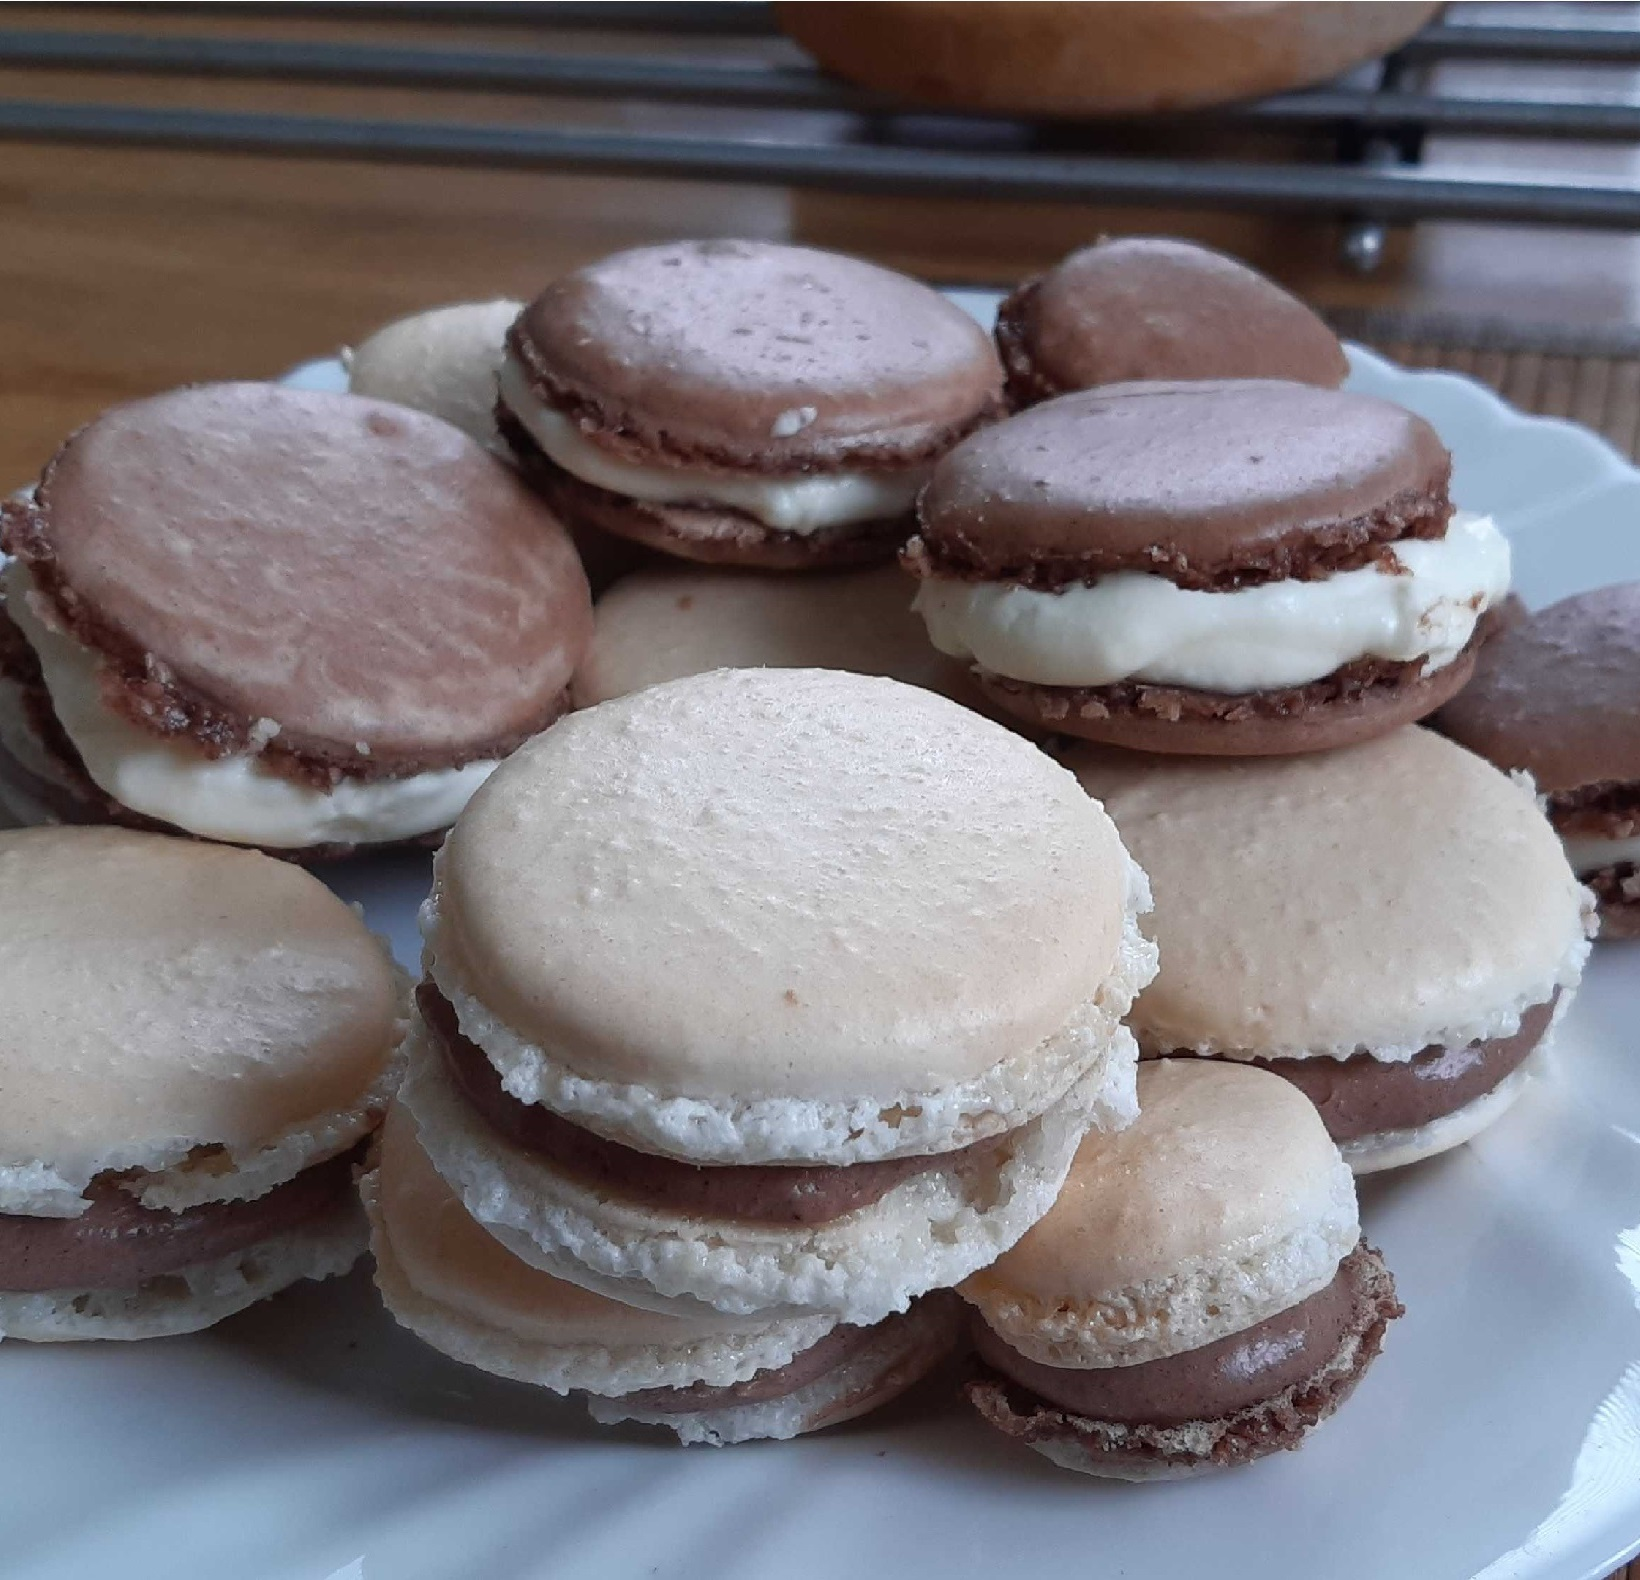
\includegraphics[height=5.5cm]{images/makronky}
  
  \def\portions{  }
  \textbf{ {\normalsize Ingrediencie (15 porcie):} }

  \begin{main}
      \item 
  \end{main}
  
    \begin{subingredient}{Cesto}
        \item 1 hrnček madľové plátky
        \item 1 hrnček práškový cukor
        \item 2 bielka
        \item 1/4 hrnčeka kryštálový cukor (treba zistiť, či naozaj treba)
        \item 2 lyžičky kakao
    \end{subingredient}
  
    \begin{subingredient}{Krém}
        \item 125ml smotana na šľahanie
        \item 200g smotanový termizovaný syr
        \item 3 lyžice práškového cukru
        \item 1 lyžica kakaa
    \end{subingredient}
  
\end{ingredient}
\begin{recipe}
\textbf{ {\normalsize Príprava:} }
\begin{enumerate}

  \item{Pripravíme krém: }
      \begin{enumerate}
          \item{Zmiešame všetko dokopy a miešame až kým to nie je tuhé}
          \item{Do polovice primiešame kakao}\end{enumerate}
  \item{Pripravíme cesto: }
      \begin{enumerate}
          \item{Bielka vymiešame do tuhého snehu}
          \item{Posekáme mandľové plátky na múku}
          \item{Preosejeme cez sitko do snehu}
          \item{Primiešame kryštálový aj práškový cukor}
          \item{Do polovice primiešame kakao}\end{enumerate}
  \item{Cesto cukrárskym vreckom nanesieme na papier na pečenie, a počkáme 20-30 minút, kým makrónky zaschnú}
  \item{Pečieme 10-15 minút pri 150°C}

\end{enumerate}
\end{recipe}

\begin{notes}
  Kakaová polovica cesta sa nejako v rúre roztiekla, neviem prečo. Celé je to fakt slané, asi by bolo zmenšiť množstvá cukru.
\end{notes}	
\clearpage
